   \begin{MyInnerSplitBox}{Year 8 and below}
     Five squares are positioned as shown. The smallest, shaded square has an area of  \(\SI{1}{\square\cm}\). What is the value of \(h\)?
     \iftoggle{SOLUTION}{%conditional output begin
      \begin{MySolutionBox}
        The shaded square has area \(\SI{1}{\square\cm}\) so it has sides of length \(\SI{1}{\cm}\).\par
        Let the length of the side of the largest square be \(a\). Then we can see that the next largest square must have side \(a-1\) because the shaded square on top of it exactly reaches to the top of the largest square. By the same reasoning the third largest square has side \(a-2\) and the smallest unshaded square has side \(a-3\). Now we can find two expressions for the distance across the diagram left to right.
        \begin{align*}
          Y &= X\\
          (a-1) + a &= (a-2) + (a-3) + h\\
          2a - 1 &= 2a -5 + h\\
          -1 &= -5 + h\\
          h &= 4
        \end{align*}
      \end{MySolutionBox}
    }{}%conditional output end
      \tcblower
      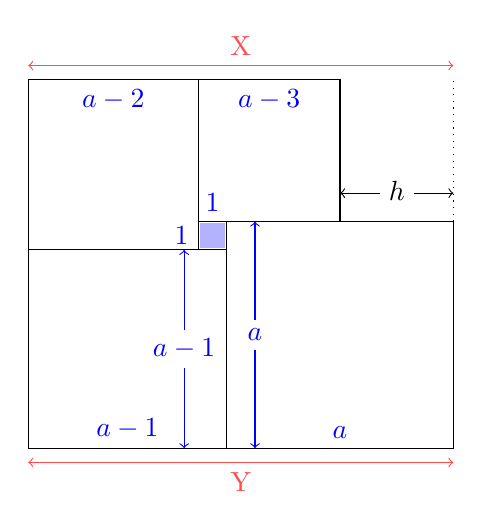
\begin{tikzpicture}[scale=0.36]
        \draw (15,0) rectangle (7,8);
        \draw (7,0) rectangle (0,7);
        \draw (0,7) rectangle (6,13);
        \draw (6,13) rectangle (11,8);
        \fill[blue!30] (6.05,7.05) rectangle (6.95,7.95);
        \draw[thin,dotted] (15,8) -- (15,13);
        \draw[<->] (15,9) -- (11,9) node[midway,fill=white,text height=0.5em] {\(h\)};
        \iftoggle{SOLUTION}{%conditional output begin
          \node[left, blue] at (6,7.5) {\(1\)};
          \node[above, blue] at (6.5,8) {\(1\)};
          \node[above, blue] at (11,0) {\(a\)};
          \node[above, blue] at (3.5,0) {\(a-1\)};
          \node[below, blue] at (3,13) {\(a-2\)};
          \node[below, blue] at (8.5,13) {\(a-3\)};
          \draw[<->,blue] (8,0) -- (8,8) node[midway,fill=white] {\(a\)};
          \draw[<->,blue] (5.5,0) -- (5.5,7) node[midway,fill=white] {\(a-1\)};
          \draw[<->,red!70] (0,-0.5) -- (15,-0.5) node[midway,below] {Y};
          \draw[<->,red!70] (0,13.5) -- (15,13.5) node[midway,above] {X};
        }{}%conditional output end
      \end{tikzpicture}
     \end{MyInnerSplitBox}

